\documentclass{epsrc}

\usepackage{lipsum} %only needed for dummy text

\usepackage[version=3]{mhchem}
\usepackage{chemstyle}
\usepackage{graphicx}
\usepackage{amsmath}
\usepackage{amsfonts}
\usepackage{array}
\usepackage{wrapfig}
\usepackage{float}

%set up different captions
\usepackage{caption}
\captionsetup[figure]{labelfont={it,bf},textfont=it}

%multiple bibliographies\
\usepackage[super,sort&compress,numbers,]{natbib}
\setlength{\bibsep}{0.0pt}

\usepackage[resetlabels]{multibib}
\newcites{A,B}{References,%
References}

%for highlighting, not needed in final
\usepackage{soul}

%to do notes, not needed in final
\usepackage[colorinlistoftodos,prependcaption,textsize=tiny]{todonotes}

\usepackage[british]{babel}

% allow use of roman numerals for lists and remove spacing
\usepackage{enumitem}
\setlist{nolistsep}

%%%Fancy header settings
\usepackage{fancyhdr}
\setlength{\headheight}{20pt}
\pagestyle{fancy}
\rhead[A. N. Other]{A. N. Other}
\lhead[Short Title, Acronym, or other Ref]%
{Short Title, Acronym, or other Ref}
\chead[]{}
\rfoot[\textbf{Draft: \today}]{\textbf{Draft: \today}}%remove in final
\cfoot[\thepage]{\thepage}

\begin{document}
\listoftodos%remove from final
\newpage% remove from final
\title{A brilliant proposal for the EPSRC prepared in \LaTeXe}
\author{A. N. Other}
\maketitle

\part{Previous track record}
\lipsum[1-5]\citeA{}
\lipsum[6-14]
\bibliographystyleA{angew}
\bibliographyA{refs}

\newpage

\part{Description of proposed research and context}

\section{Vision, Aims and Context of the fellowship}

\lipsum[15-16]

\section{Adventure and potential impact}

\lipsum[17-18]

\begin{enumerate}[label=\roman*.]
	\item A
	\item B
	\item B
\end{enumerate}

\section{Research Concept}

\begin{figure}[!htbp]
	\begin{center}
		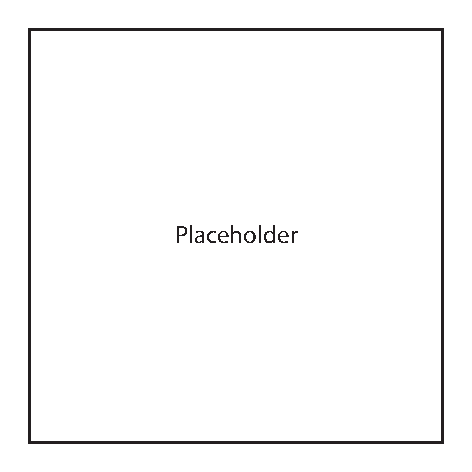
\includegraphics{img/placeholder_image}
		\vspace{-30pt}
		\caption{some caption}
		\label{fig:full}
	\end{center}
\end{figure}

\lipsum[19-20]

\begin{itemize}
	\item[-]A
	\item[-]B
	\item[-]C
\end{itemize}

\section{Background and Context}

\lipsum[21-22]\hl{highlight bits of text}

\begin{enumerate}[label=\bfseries \arabic*:, align=left]
	\item A
	\item B
	\item C
\end{enumerate}

\lipsum[23-24]

\begin{enumerate}[label=\bfseries Objective \arabic*:, align=left]
	\item A
	\item B
	\item B
	\item C
\end{enumerate}

\lipsum[25-26]\citeB{}

\begin{wrapfigure}{r}{0.5\textwidth}
\vspace{-11pt}
	\begin{center}
		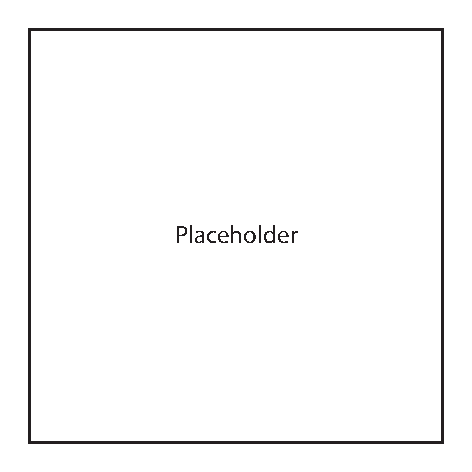
\includegraphics[width=8.5cm]{img/placeholder_image}
			\vspace{-30pt}
		\caption{A half width figure}
		\label{fig:half}
	\end{center}
\end{wrapfigure}

\lipsum[27-30]\todo{use to-do notes for annotations}


\bibliographystyleB{angew}
\bibliographyB{case4support} %your .bib file
\end{document}
